% For instructions, 
\documentclass{article}
\usepackage[utf8]{inputenc}
\usepackage{amsmath}
\usepackage{listings}
\usepackage{geometry}
\usepackage{graphicx}
\usepackage{subfig}
\usepackage[colorlinks=true]{hyperref}
\usepackage{dcolumn}% Align table columns on decimal point
\usepackage{bm}% bold math
\usepackage{hyperref}% add hypertext capabilities
\usepackage{booktabs}
\usepackage{gensymb}
\footskip = 90pt
\begin{document}

\title{%
  The Apex of Coffee Containment \\
  \large Obligatory Assignment 1 \\
  FYS2160 at the University of Oslo}
%In a multipart project you may find a title that covers the common aspects of what you present


\author{Simen Løken}


\date{\today}
\maketitle
\begin{abstract}
In this assignment we'll be looking at the decently popular Temperfect mug, and how it works on a macro-/microscopic level. We'll be comparing data to our numerical, analytic and theoretical solutions, and we end of finding that an Einstein model fits our model well.
\end{abstract}





\section{Introduction}
The Temperfect mug was a Kickstarter project successfully funded in the latter part of 2013. Although not an entirely new concept, as a "phase-shift" mug had been proposed and patented all the way back in the 1960s \cite{article}, it gained a fair bit of media traction and has since become the Alpha and Omega for any coffee-enthusiast looking to "up their game", but how does it work, and why?
\section{Results and discussion}
First we use the data provided in termokopper.txt to plot the temperature in our mugs over just under 7000 seconds:
\begin{figure}[ht]
    \centering
    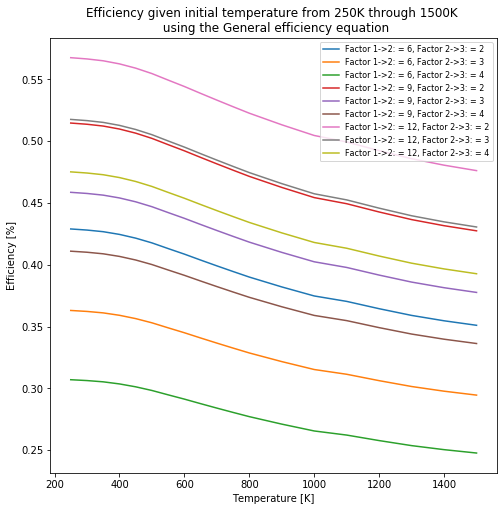
\includegraphics[scale=0.5]{figure1.png}
    \caption{Temperature of liquid over time}
    \label{fig:1}
\end{figure}
\newpage
We see that Mug A follows a steady decline towards the room temperature of about 20\degree C. Mug A is not very interesting, so I will instead be talking about Mug B.\newline
We see that Mug B very rapidly goes down to about 65\degree C which is pretty close to the ideal temperature for coffee (coming from someone who doesn't drink coffee). This alone tells us that Mug B is the Temperfect mug, as when the warm liquid enters the container, it melts the metal contained in-between the "walls" of the Temperfect mug. As this liquid becomes solid again, it exudes heat which is then used to "reheat" the warm liquid in the container, keeping it at ideal temperatures for longer than a normal mug
\newline
Another point of interest for Mug B is at about 2200~ seconds, where Mug B starts to follow Mug A's steady decline towards the room temperature. This is because all of the "wall"-liquid has now gone back to being a solid, which means it no longer exudes any heat. I'm assuming it'd last a lot longer if the lid was on.
\newline
Let's look at why this works, and how material behaves when phase-shifting.
When considering the phase-shift of a material, we can express it's entropy given temperature as:
\begin{figure}[ht]
    \centering
    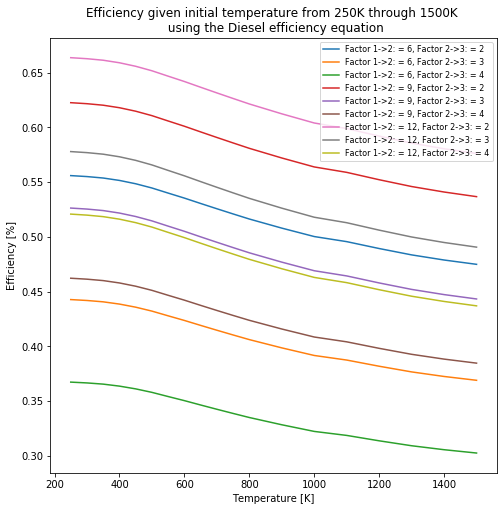
\includegraphics[scale=0.5]{figure2.png}
    \caption{Entropy of a material as temperature increases}
    \label{fig:2}
\end{figure}
\newline
Section I is our solid phase, here our entropy increases "sort-of" proportionally to our temperature, but not quite. As we then reach the first * and into Section II, we experience a phase-shift into liquid form, and as such our entropy increases pretty drastically since our material now has a lot more freedom to freely move around, instead of being constrained to neighbouring molecules (at least to the same degree). We then approach our second phase-shift, which elevates us even higher than our previous phase-shift did.
\newline
An interesting take-away from this is that this also works in reverse, and this is what makes the Temperfect work. As the heat from our, let's say coffee, heats our mystery-wall-material, which causes it to melt, absorbing excess heat above it's melting point, preferably around "drinkable" temperatures of 60-70\degree C. It then exudes this heat creating a sort-off equilibrium between itself and the coffee. When all of our wall-material has gone back to being a solid, the effect stops working, and the mug becomes a normal mug again.
\newpage
We're going to try to model this using an Einstein solid, whose internal energy we can express as:
\begin{equation} \label{1}
    U= \frac{N'\epsilon}{2}+q\epsilon
\end{equation}
\newline
where $N'=3N$, aka our harmonic oscillators, given by their three degrees of freedom. \newline
The multiplicity of such a system can then be expressed as
\begin{equation} \label{4}
    \Omega = \frac{(q+N'-1)!}{q!(N'-1)!}
\end{equation}
\newline
This of course also means that we can now find an expression for our entropy as:
\begin{equation*}
    S = k_B ln \Omega = k_B ln \frac{(q+N'-1)!}{q!(N'-1)!}
\end{equation*}
\newline
This equation is fine, but ideally we'd simplify it a bit. Assuming N' is sufficiently large, the -1 should be irrelevant and thus we get:
\begin{equation*}
    \frac{S}{k_B} = ln \frac{(q+N')!}{q!N'!}
\end{equation*}
Using Stirling Approximation we can rewrite this as:
\begin{equation} \label{2}
     \frac{S}{k_B} \approx (q+N')ln(q+N')-N' ln N'-q ln q
\end{equation}
Temperature can be expressed as:
\begin{equation*} 
    \frac{1}{T} = \frac{\delta S}{\delta U} = \frac{k_B}{\epsilon} ln(1+\frac{N'}{q})
\end{equation*}
\begin{equation}\label{3}
    T = (\frac{\delta S}{\delta U} = \frac{k_B}{\epsilon} ln(1+\frac{N'}{q}))^{-1}
\end{equation}
Finally, using Eq. \ref{1}, Eq. \ref{2} and Eq. \ref{3} we can eliminate q and find that:
\begin{equation}
    U = \frac{N' \epsilon}{2} + \frac{N' \epsilon}{(e^{\frac{\epsilon}{k_BT}}-1)^2}
\end{equation}
If we now differentiate in respect to temperature we can find that $C_V$ is:
\begin{equation}
    C_V = \frac{\delta U}{\delta T} = \frac{N' \epsilon^2}{k_BT^2} \frac{e^{\frac{\epsilon}{k_BT}}}{(e^{\frac{\epsilon}{k_BT}}-1)^2}
\end{equation}
\newpage
Let's now assume we've got the values $N = 400$ and $q = 200$. We can make a plot of our model to see how the heat capacity changes with temperature:
\begin{figure}[ht]
    \centering
    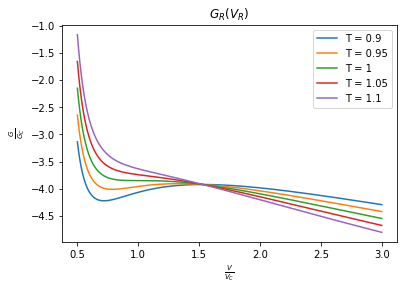
\includegraphics[scale=0.5]{figure3.png}
    \caption{Heat capacity for temperatures 50-400 K}
    \label{fig:3}
\end{figure}
\newline
I chose a frequency of $1420.4\times10^6$ Hz, the frequency of Hydrogen, but I could've chose anything frankly, so long as it gives a nice curve. The interesting thing to note is that it very closely resembles Figure 1.14 from \cite{schroeder_daniel_thermal_physics}, at least the curve for lead.
\newline
This at least tells us that for smaller values of $f$ and as a result, $\epsilon$ we get steeper heat capacity model. As such, we can estimate that $\epsilon_{Pb} < \epsilon_{Al} < \epsilon_{C}$
\newline
Let's now derive another way to express the multiplicity of an Einstein solid. We have Eq. \ref{4} which we can then rewrite as:
$$\Omega = \frac{(q+N'-1)!}{q!(N'-1)!} \newline$$
$$\Omega = \frac{1}{q!} \frac{N}{N!} \frac{(q+N)!}{(q+N)}$$
$$\Omega = \frac{N}{q+N} \frac{(q+N)!}{q!N!}$$
We can then use Stirling Approximation and get:
$$\Omega \approx \frac{N}{q+N} \frac{\sqrt{2\pi (q+N)} (q+N)^{q+N} e^{-(q+N)}}{2\pi \sqrt{qN}q^q N^N e^{-(q+N)}}$$
Which looks incredibly ugly, but can be simplified to be:
\begin{equation}
    \Omega \approx  (\frac{q+N}{q})^2 (\frac{q+N}{N})^2 \sqrt{\frac{N}{2\pi q(q+N)}}
\end{equation}
It is sometimes beneficial to ignore the root, and as such, we can also write:
\begin{equation}
    \Omega \approx  (\frac{q+N}{q})^2 (\frac{q+N}{N})^2
\end{equation}
\section{Methods}
For this experiment we've used two steel thermo mugs, two thermometers and a "translator" that'll read our data and plug it into a .txt file for further use. Additionally we've used some code, which is included in the delivery.
\section{Conclusion}
Now of course, the question on everyone's minds is whether or not we can use an Einstein model to model the Temperfect mug. In my opinion we can. We show that it is easier to warm up an cold Einstein Solid, in our case the mystery-wall-material, and that as the temperature increases it's harder to continue heating up the mystery-material. This is what prevents all our coffee-heat from rushing into the walls. When the "resistance", or rather, heat capacity becomes high enough, our system forms an equilibrium between the coffee and the mystery-material, only occasionally transferring heat to the coffee to maintain the equilibrium until all the excess heat stored in the wall-material is gone.
\newline
So yes, I do think the Einstein solid makes for an excellent model as to why this works on a macro/micro-level.


\bibliographystyle{unsrt}
\bibliography{Bibliography.bib}
\clearpage

\appendix

\section{Requested problems}
\subsection{Finding expressions}
\begin{itemize}
    \item S(U,N) \newline
\begin{equation}
    \Omega = \frac{(q+N'-1)!}{q!(N'-1)!}
\end{equation}
\newline
For simplicity's sake, let's approximate this equation. We then get:
\begin{equation}
    ln \Omega = (q+N)ln(q+N) - qlnq - NlnN
\end{equation}
If we assume that $q >> N$, we can further simplify this to be:
\begin{equation}
    \Omega \approx (\frac{q}{N})^N
\end{equation}
The complete derivation for this can be found in \cite{comp}. \newline
This of course also means that we can now find an expression for our entropy as:
\begin{equation*}
    S(U,N) = Nk_B lnU - Nk_B ln(\epsilon N) + Nk_B
\end{equation*}
    \item T(U,N) \newline
    Following above, we can derive T to be:
    \begin{equation}
        \frac{1}{T} = \frac{\delta S}{\delta U} = \frac{Nk_B}{U}
    \end{equation}
    \begin{equation}
        T(U,N) = \frac{U}{Nk_B}
    \end{equation}
    \item $C_V$(T,N) \newline
    This was shown when finding the heat capacity of the Einstein solid, and is:
    \begin{equation}
    C_V(N,T) = 3Nk_B (\frac{\epsilon}{k_BT})^2 \frac{e^{\frac{\epsilon}{k_BT}}}{(e^{\frac{\epsilon}{k_BT}}-1)^2}
\end{equation}
    \item $c_V$(T) \newline
    The molar heat capacity is given as:
    \begin{equation}
        c_V(T) = \frac{C_V(N,T)}{n}
    \end{equation}
    where n is the number of moles.
\end{itemize}



\end{document}
